\let\negmedspace\undefined
\let\negthickspace\undefined
\documentclass[journal]{IEEEtran}
\usepackage[a5paper, margin=10mm, onecolumn]{geometry}
\usepackage{tfrupee} 
\setlength{\headheight}{1cm} 
\setlength{\headsep}{0mm}     

\usepackage{gvv-book}
\usepackage{gvv}
\usepackage{cite}
\usepackage{amsmath,amssymb,amsfonts,amsthm}
\usepackage{algorithmic}
\usepackage{graphicx}
\usepackage{textcomp}
\usepackage{xcolor}
\usepackage{txfonts}
\usepackage{listings}
\usepackage{enumitem}
\usepackage{mathtools}
\usepackage{gensymb}
%\usepackage{wasysym}
\usepackage{comment}
\usepackage[breaklinks=true]{hyperref}
\usepackage{tkz-euclide} 
\usepackage{listings}
\def\inputGnumericTable{}                                 
\usepackage[latin1]{inputenc}                                
\usepackage{color}                                            
\usepackage{array}                                            
\usepackage{longtable}                                       
\usepackage{calc}                                             
\usepackage{multirow}                                         
\usepackage{hhline}                                           
\usepackage{ifthen}                                           
\usepackage{lscape}
\usepackage{circuitikz}
\tikzstyle{block} = [rectangle, draw, fill=blue!20, 
    text width=4em, text centered, rounded corners, minimum height=3em]
\tikzstyle{sum} = [draw, fill=blue!10, circle, minimum size=1cm, node distance=1.5cm]
\tikzstyle{input} = [coordinate]
\tikzstyle{output} = [coordinate]
\renewcommand{\thefigure}{\theenumi}
\renewcommand{\thetable}{\theenumi}
\setlength{\intextsep}{10pt} % Space between text and floats
\numberwithin{equation}{enumi}
\numberwithin{figure}{enumi}
\renewcommand{\thetable}{\theenumi}

\begin{document}

\bibliographystyle{IEEEtran}
\vspace{3cm}

\title{10.4.8}
\author{EE25BTECH11032 - Kartik Lahoti}
\maketitle

\subsection*{Question: } 
For which value of $m$ is the line
\begin{align}
    y = mx + 1
\end{align}
a tangent to the curve 
\begin{align}
    y^2 = 4x
\end{align}

\textbf{Solution}:\\

Given parabola 
\begin{align}
    g\brak{\vec{x}} = \vec{x}^{\top}\vec{V}\vec{x} + 2\vec{u}^{\top}\vec{x} + f = 0 \\
    \vec{V} = \myvec{0&0\\0&1} , \vec{u} = \myvec{-2\\0} , f = 0.
\end{align}
Given Line equation
\begin{align}
    \vec{x} = \vec{h} + k\vec{m}\\
    \vec{h} = \myvec{0\\1} , \vec{m} = \myvec{1 \\ m}.
\end{align}

For the line to be a tangent , all the solution for $k$ should be equal

\begin{align}
    k_i = \frac{1}{\vec{m}^{\top}\vec{V}\vec{m}}\brak{-\vec{m}^{\top}\brak{\vec{V}\vec{h}+\vec{u}} \pm \sqrt{\sbrak{\vec{m}^{\top}\brak{\vec{V}\vec{h}+\vec{u}}}^2-g\brak{\vec{h}}\brak{\vec{m}^{\top}\vec{V}\vec{m}}}} \label{eq_1}
\end{align}

From \ref{eq_1} 
\begin{align}
    \sbrak{\vec{m}^{\top}\brak{\vec{V}\vec{h}+\vec{u}}}^2 = g\brak{\vec{h}}\brak{\vec{m}^{\top}\vec{V}\vec{m}} \label{eq_3}
\end{align}

\begin{align}
    g\brak{\vec{h}} = \myvec{0&1}\myvec{0&0\\0&1}\myvec{0\\1} + 2\myvec{-2&0}\myvec{0\\1} + 0 = 1 \label{eq_2}
\end{align}

Using \ref{eq_2} in \ref{eq_3}

\begin{align}
    \sbrak{\myvec{1 & m }\brak{\myvec{0&0\\0&1}\myvec{0\\1} + \myvec{-2\\0}}}^2 = 1\brak{\myvec{1&m}\myvec{0&0\\0&1}\myvec{1\\m}}
\end{align}

\begin{align}
    \implies \brak{m-2}^2 &= m^2 \\ 
    \implies 4 - 4m &=   0 \\ 
    \implies m &= 1
\end{align}

\begin{figure}[H]
    \centering
    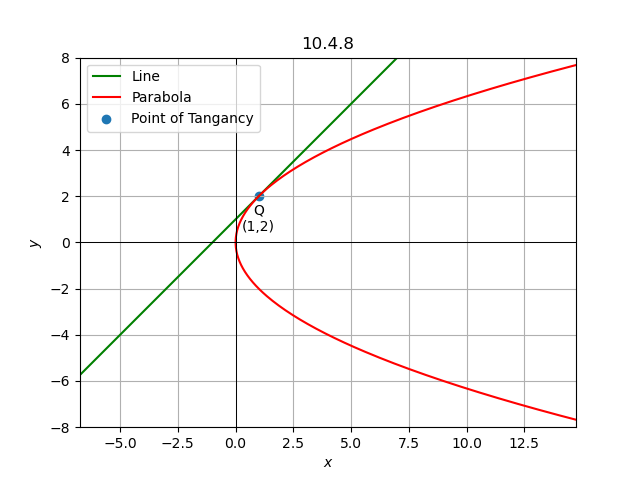
\includegraphics[width=1\columnwidth]{figs/graph2.png}
    \caption*{}
    \label{fig:placeholder}
\end{figure}

\end{document}


